\documentclass[12pt, french]{article}
\usepackage{mhchem}
\usepackage{fancyhdr, fancybox, lastpage, makecell}
\usepackage[most]{tcolorbox}
\usepackage[a4paper, margin={0.3in, .75in}]{geometry}
\usepackage{wrapfig}
\pagestyle{fancy}
\renewcommand\headrulewidth{1pt}
\renewcommand\footrulewidth{1pt}
\fancyhf{}
\rhead{ \em{Zakaria Haouzan}}
\lhead[C]{\em{2ème année baccalauréat SM-X}}
\chead[C]{}
\rfoot[C]{}
\lfoot[R]{ \emph{Exercices Supplémentaires}}
\cfoot[]{\em{Page \thepage / \pageref{LastPage}}}


\newtcolorbox{Box2}[2][]{
                lower separated=false,
                colback=white,
colframe=white!20!black,fonttitle=\bfseries,
colbacktitle=white!30!gray,
coltitle=black,
enhanced,
attach boxed title to top left={yshift=-0.1in,xshift=0.15in},
title=#2,#1}


\begin{document}
\begin{center}
   \shadowbox {\bf{Suivi d’une transformation chimique }}
\end{center}

\vspace{-0.2cm}
%%_________________________Exercice ! :"_________________________Exercice
%   \begin{center}
	   %\vspace{-0.6cm}
	%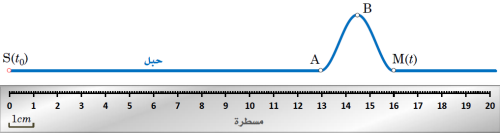
\includegraphics[width=0.6\textwidth ]{./img/Exercice01.png}
  %\end{center}
%\begin{wrapfigure}[2]{r}{0.48\textwidth}
  %\begin{center}
	  %\vspace{-1cm}
	%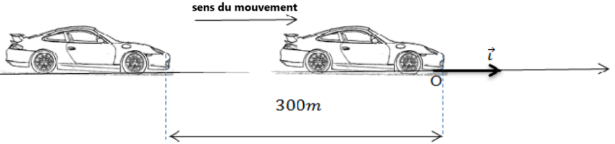
\includegraphics[width=0.48\textwidth]{./img/ex1.png}
  %\end{center}
%\end{wrapfigure}
%\begin{tcolorbox}\textbf{Exercice 2 : propagation d’ondes ultrasonores et des ondes lumineuses }
%\end{tcolorbox}





\begin{Box2}{\textbf{Exercice 1 :comprimé d'aspirine}}
\begin{wrapfigure}[7]{r}{0.48\textwidth}
  \begin{center}
	  \vspace{-1cm}
	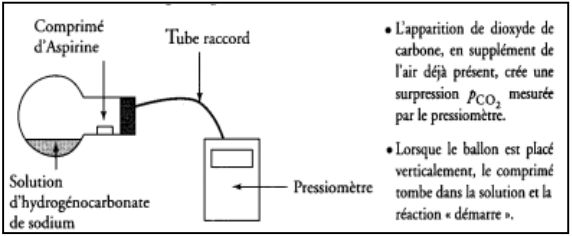
\includegraphics[width=0.48\textwidth]{./img/ex01_1.png}
  \end{center}
\end{wrapfigure}

	Un comprimé d'aspirine effervescent est mis dans un verre d'eau. Entre l'aspirine, principe actif du
médicament, et l'ion hydrogénocarbonate $HCO_3^-$ , se produit une réaction dont l'équation est :
${C_9H_8O_4}_{(aq)} + {HCO_3^-}_{(aq)} \rightarrow {C_9H_7O_4^-}_{(aq)} + {CO_2}_{(g)} + H_2O_{(l)}$.

\underline{Dans tout l'exercice, elle sera considérée comme totale}.

\textbf{1. }On envisage de reproduire la réaction
précédente au laboratoire en mettant
en contact un comprimé d'aspirine $500$
non effervescent, qui contient donc
$500mg$ de principe actif et une solution
d'hydrogénocarbonate de sodium.

Le dispositif expérimental d’étude est
schématisé ci-contre. Le dioxyde de
carbone produit sera considéré comme un gaz parfait.

\begin{itemize}

	\item Le volume total de l’enceinte est : $V= 310 mL$ et la température de l’expérience est : $\theta=26,0^{\circ}C$.
	\item La constante des gaz parfaits est : $R = 8,31 SI$.
	\item  $M(C_9H_8O_4)=180g/mol$
\end{itemize}
La solution d'hydrogénocarbonate de sodium $({Na^+}_{(aq)}+ {HCO_3^-}_{(aq)})$ introduite dans le ballon a un volume
$V_1=10mL$ et une concentration molaire en soluté apporté : $C_1=0,500 mol.L^{-1}$.

\textbf{Vérifier que la solution introduite permet la
consommation totale de l'aspirine contenue dans
un comprimé.}

\begin{wrapfigure}[9]{r}{0.48\textwidth}
  \begin{center}
	  \vspace{-1.2cm}
	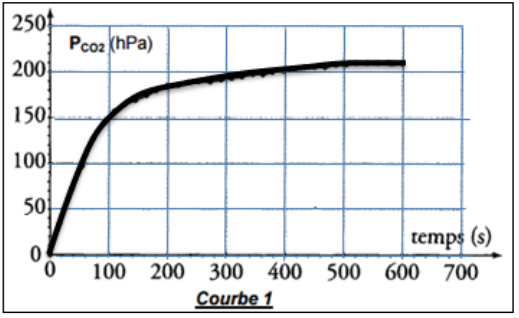
\includegraphics[width=0.48\textwidth]{./img/ex01_2.png}
  \end{center}
\end{wrapfigure}

\textbf{2. }La réaction est suivie par une méthode
physique : mesure de la pression à
l'intérieur d'une enceinte étanche.

Le suivi expérimental de la surpression $P_{CO_2}$,
provoquée par l’apparition du dioxyde de
carbone dans l’enceinte étanche, donne lieu à la
Courbe 1 ci-contre. Montrer que l’on a
sensiblement la relation numérique suivante donnant la quantité de matière de dioxyde de carbone formé :

$n_{CO_2} = 1,21.10^{-7}.P_{CO2}$.

Préciser les unités intervenant dans cette formulation.

\textbf{3. }Construire le tableau d’avancement de la transformation chimique étudiée.

\textbf{4. }Exprimé la vitesse instantanée de la réaction en: $\frac{dP_{CO_2}}{dt}$

\textbf{5. }Déterminer une valeur numérique de cette vitesse à l’instant $t = 0 s$.

\textbf{6. }Établir la relation entre la quantité de dioxyde de carbone formée, n(CO2), et la quantité d'aspirine
consommée, $n_{asp}$

\textbf{7. }Calculer la masse d'aspirine contenue dans le comprimé.

\textbf{8. }Comparer à la valeur indiquée par le fabricant en calculant un pourcentage d’écart. Conclure.

\textbf{9. } On refait la même expérience mais à température T=40°C, tracer, en justifiant, sur la même courbe
précédente, l’allure de la courbe obtenue dans ce cas.

\end{Box2}

%\vspace{1.6cm}

\begin{Box2}{Exercice 2 :L’eau de Javel }
L’eau de Javel se décompose lentement selon la réaction d’oxydoréduction suivante :
$$2ClO^-_{(aq)} \rightarrow 2Cl^-_{(aq)} + {O_2}_{(g)}$$
On utilise de l’eau de Javel achetée en berlingot de degré chlorométrique 48°. On dilue la solution
commerciale afin d’obtenir une solution $S_1$ cinq fois moins concentrée. Pour étudier la cinétique de cette
réaction de
décomposition catalysée, on utilise un volume $V_1 = 100 mL$ de la solution $S_1$. 

On déclenche le chronomètre
à l’instant où l’on met le catalyseur dans la solution. Pour suivre l’évolution de la réaction, on mesure à
température et pression constantes le volume de dioxygène dégagé au cours du temps. Dans le graphe ci-contre, le volume de dioxygène dégagé $V(O_2)$ est
déterminé à la température de 20°C et sous la
pression de 1013 hPa.

\textbf{1. }Faire un schéma de l'expérience qui permet de
suivre l'évolution de cette transformation

\textbf{2.} Dresser le tableau d’avancement de cette
transformation.

\textbf{3. } Déterminer la valeur de l’avancement maximal $x_{max}$ et déduire la quantité de matière initiale de
$ClO^-$ dans la solution $(S_1)$.

\textbf{4. } Calculer la concentration initiale $C_1$ de $(S_1)$ puis déduire la concentration $C_0$ de $(S_0)$.

\textbf{5. }Vieillissement de l’eau de Javel.

Le degré chlorométrique correspond au volume de dichlore gazeux en L, mesuré à 0° C et sous 105 Pa
nécessaire à la préparation d’un litre d’eau de Javel suivant une transformation totale modélisée par
l’équation suivante : 

$${Cl_2}_{(g)} + 2 {HO^-}_{(aq)} \rightarrow {H_2O}_{(aq)} + Cl^-_{(aq)} + ClO^-_{(aq)}$$

\textbf{5.1. } Calculer le degré chlorométrique de l’eau de Javel utilisée pour l’expérience, en remarquant
qu’au bout de $450s$, tous les ions hypochlorites ont été consommés.

\textbf{5.2. }Comparer cette valeur à celle qui est fournie par le fabricant et conclure.

\textbf{6. }La vitesse de la réaction

\textbf{6.1. }Ecrire l’expression de la vitesse volumique à un instant t, en fonction de $\frac{dV(O_2)}{dt}$

\textbf{6.2.}Déterminer la vitesse de la réaction à $t =0 s$ et $t = 300 s$, Comment évolue la vitesse volumique au cours du temps ? donner une explication.

\textbf{7. }Définir le temps de demi-réaction $t_{1/2}$ et donner sa valeur.
  \begin{center}
	  %\vspace{-1.2cm}
	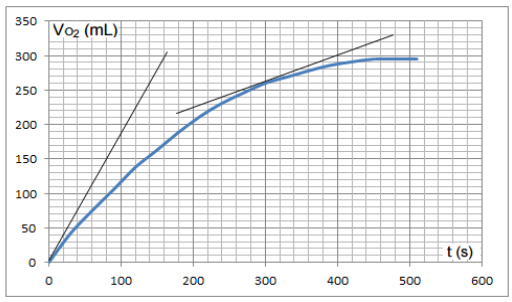
\includegraphics[width=0.48\textwidth]{./img/ex2.png}
  \end{center}
\end{Box2}


\begin{Box2}{Exercice 3 :La cinétique de l’hydrolyse basique (saponification) }
\emph{Le but de cet exercice est d’étudier la cinétique de l’hydrolyse basique (saponification) d’un ester (E) de
formule, $CH_3COOC_2H_5$ suivi par conductimétrie.}

On mélange rapidement dans un bécher une quantité $n_1 =0,010 mol$ d’hydroxyde de sodium $(Na^+$+$HO^-)$ et une quantité $n_2$ de l’ester en excès, à $25 ^{\circ}C$. Une réaction lente d’équation :

$${CH_3COOC_2H_5}_{(aq)} + {HO^-}_{(aq)} \rightarrow {CH_3COO^-}_{(aq)} +  {C_2H_5OH}_{(aq)}$$


\begin{wrapfigure}[7]{r}{0.48\textwidth}
  \begin{center}
	  %\vspace{-1.2cm}
	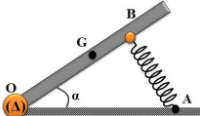
\includegraphics[width=0.48\textwidth]{./img/ex03.png}
  \end{center}
\end{wrapfigure}

Se déroule dans le bécher. Cette réaction d’hydrolyse de l’ester est considérée comme une transformation
chimique totale. 

On note V le volume total du mélange réactionnel.

\textbf{Données : } 
\begin{itemize}
	\item On appelle constante de cellule le rapport
de la conductance G et de la conductivité de la
solution $\sigma$. On peut donc écrire la relation 

$G$=$ k . \sigma$

\item Conductivités molaires ioniques de quelques ions 25°C en $S.m^2. mol^{ -1}$: 

	$\lambda(Na^+) $=$ 5,01.10^{-2}$ ; $\lambda(HO^-) $=$ 1,99.10^{-2}$ ; $\lambda(CH_3CO2^-)= 4,09.10^{-3}$
\end{itemize}

\textbf{1- Étude de la conductance G : }
À l’aide d’un conductimètre, on mesure la
conductance G du mélange réactionnel au cours du
temps (Figure ci-contre).

\textbf{1.1. }Expliquer la diminution de la conductance mesurée au cours de la transformation chimique.

\textbf{1.2} Dresser le tableau d’avancement de la réaction chimique.

\textbf{1.3. }Donner l’expression de la conductance initiale $G_0$ (à t= 0) en fonction de k, $n_1$, V et des conductivités
molaires ioniques.

\textbf{1.4. } Donner l’expression de la conductance G, à chaque date t, en fonction de x , k, $n_1$, V et des
conductivités molaires ioniques, où x est l’avancement de la réaction à la date t.

\textbf{1.5. } Donner l’expression de la conductance $G_f$ au bout d’un temps très long.

\textbf{1.6} Établir la relation suivante : x = $n_1.\frac{G_t - G_0}{G_f - G_0}$ et Déterminer $t_{1/2}$ le temps demi-réaction.


\end{Box2}

\begin{tcolorbox}\textbf{Exercice 4 :l’évolution de la réaction de l’acide butanoïque avec le méthanol }
\end{tcolorbox}
De la réaction de l’acide butanoïque avec le méthanol résulte un composé organique E et de l’eau.
Cette réaction est modélisée par l’équation suivante.

$$\ce{C_3H_7COOH + CH_3OH <=> C_3H_7COOCH_3 + H_2O}$$


\textbf{1. }On verse dans un ballon se trouvant dans un bain d’eau glacée :
\begin{itemize}
	\item $n_1$ = 0,1 mol d’acide butanoïque ;

	\item $n_2$ = 0,1 mol de méthanol ;
	\item Quelques gouttes d’acide sulfurique concentré ;

	\item Quelques gouttes de phénolphtaléine.
	\item On obtient ainsi un mélange de volume V = 400 mL.
\end{itemize}
Quel est l’intérêt de l’utilisation de l’eau glacée et le rôle de l’acide sulfurique dans cette réaction ?

\begin{wrapfigure}[11]{r}{0.48\textwidth}
  \begin{center}
	  \vspace{-1.2cm}
	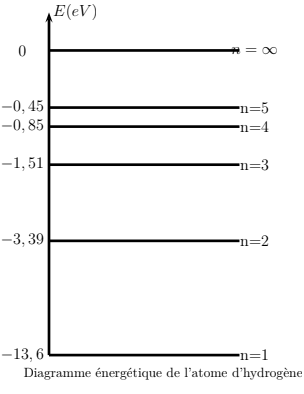
\includegraphics[width=0.48\textwidth]{./img/ex04.png}
  \end{center}
\end{wrapfigure}



\textbf{2. }Pour suivre l’évolution de cette réaction, on répartit le mélange sur 10 tubes à essai, qu’on ferme et
on place dans un bain marie de température maintenue constante (100°C), et on déclenche un
chronomètre au même instant choisi comme origine des dates t = 0.

Pour déterminer l’avancement de la réaction, on sort du bain marie, les tubes à essai l’un après
l’autre, on verse le contenu dans un bécher contenant de l’eau glacée, et on neutralise l’acide restant
dans chaque tube à l’aide d’une solution d’hydroxyde de sodium de concentration molaire $C = 1mol.L^{-1}$. La réaction modélisant ce dosage s’écrit comme suit:

$$\ce{AH_{(aq)} + HO^-_{(aq)} <=> A^-_{(aq)} + H_2O_{(aq)}}$$

Montrer que l’expression de l’avancement x de la réaction d’estérification à un instant t s’écrit : $$x(mol)=0,1 - (10.C.V_{BE})$$.

\vspace{-0.8cm}
Où $V_{BE}$ désigne le volume d’hydroxyde de sodium
ajouté pour atteindre l’équivalence dans chaque tube.

\textbf{2.1.}Les résultats expérimentaux de ce dosage ont
permis de tracer la courbe représentative de
l’avancement x de la réaction d’estérification
en fonction du temps
La droite (T) représente la tangente à la courbe
à l’instant t = 0.

A l’aide de ce graphe, déterminer :

\textbf{2.1.a }La vitesse volumique de la réaction
aux instant $t_0 = 0$ et $t_1 = 50 min$.

\textbf{2.1.b}Le temps de demi-réaction $t_{1/2}$.

\begin{Box2}{Exercice 5 : Suivi temporel d’une transformation
chimique}

On mélange dans un erlenmeyer un volume $V_A$=$ 11 mL$ de l’acide (A) et 0,12 mol de l’alcool
(B) On ajoute au mélange quelques gouttes
d’acide sulfurique concentré et quelques
pierres ponces. Après chauffage, il se forme un
composé ( E )
Le graphe $x = f (t)$ donne l’évolution de
l’avancement x de la réaction en fonction du
temps t, (fig1).
La droite $(\Delta)$ représente la tangente à la courbe
$x = f (t)$ à l’instant t = 0
\begin{enumerate}
	\item  Déterminer l’avancement final de la
réaction,
\item Donner la définition du temps de demi-réaction et déterminer sa valeur
\item  Calculer graphiquement la valeur de la vitesse volumique v(0) à l’instant t = 0
\end{enumerate}
  \begin{center}
	  %\vspace{-1.2cm}
	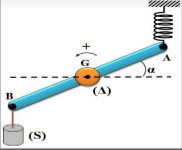
\includegraphics[width=0.48\textwidth]{./img/ex05.png}
  \end{center}

\end{Box2}

\begin{Box2}{Exercice 6 : Suivi temporel d’une transformation
chimique}
On prépare, à l'instant $t_0 = 0$ , huit $(08)$ tubes à essais numérotés de 1 à 8 et on introduit dans chacun d'eux $n_1$=$0,10 mol$ d'acide carboxylique (A), $n_2$=$0,10 mol$ de menthol et quelques gouttes d'acide sulfurique
concentré. 

On trempe, en même temps, les huit $(08)$ tubes dans un bain marie à la température constante 70°C et on déclenche le chronomètre. 

Le dosage d'acide restant dans chaque tube, à intervalles de temps réguliers,permet de déterminer la quantité de matière d'ester formé.
On modélise la réaction d'estérification entre l'acide carboxylique (A) et le menthol par l'équation chimique
suivante :
$$\ce{RCOOH_{(l)} +C_{10}H_{19}OH_{(l)} <=> C_{12}H_{22}O_2 + H_2O}$$

\textbf{1- Dosage de l'acide carboxylique (A)
restant dans le tube 1}

Au premier intervalle du temps, on retire le tube
1 du bain marie et on le trempe dans de l'eau
glacée puis on dose l'acide restant dans le
système chimique par une solution aqueuse
d’hydroxyde de sodium $Na^+_{(aq)}$+$HO^-_{(aq)}$ de
concentration molaire $C_B = 1,0 mol.L^{-1}$ en
présence d'un indicateur coloré approprié. 

Le volume ajouté à l'équivalence est $V_{BE} =68 mL$

\textbf{1.1. } Écrire l'équation de la réaction,
considérée comme totale, qui a eu lieu
au cours du dosage.

\textbf{1.2. }Montrer que la quantité de matière d'acide restant dans le tube 1 est $n_A$=$6,8.10^{-2} mol$.

\textbf{1.3. }Déterminer la valeur de la quantité de matière d'éthanoate de menthyle formée dans le tube 1. (On peut
exploiter le tableau d'avancement de la réaction étudiée)

\begin{wrapfigure}[16]{r}{0.58\textwidth}
  \begin{center}
	  \vspace{-1.2cm}
	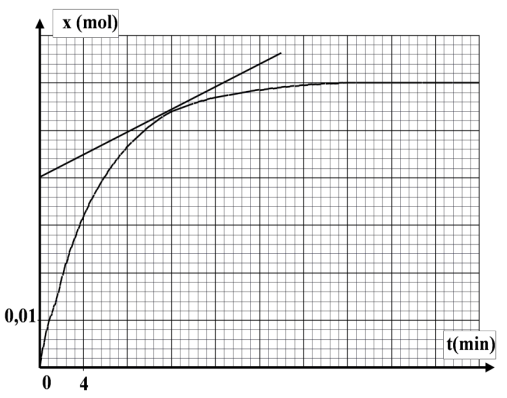
\includegraphics[width=0.58\textwidth]{./img/ex06.png}
  \end{center}
\end{wrapfigure}


\textbf{2. }Suivi temporel de la quantité de matière d'éthanoate de menthyle synthétisé Le dosage de l'acide restant dans les autres tubes à essai a permis de tracer la courbe d'évolution de
l'avancement de la réaction en fonction du temps.

\textbf{3.1. }Calculer en $(mol.L^{-1}.min^{-1})$, la valeur de la vitesse volumique de réaction aux instants $t_1 = 12 min$ et $t_2 = 32min$. sachant que le volume du système chimique est $V = 23 mL$ . 

Expliquer qualitativement la variation de cette vitesse.


\textbf{3.2. }Citer un facteur cinétique permettant d'augmenter la vitesse volumique de réaction sans changer
l'état initial du système chimique.

\textbf{3.3. }Déterminer graphiquement: 

\textbf{3.3.a. }la valeur de l’avancement final $x_f$

\textbf{3.3.b. }le temps de demi-réaction $t_{1/2}$
\end{Box2}


\begin{Box2}{Exercice 7 : la cinétique de la dissociation du pentaoxyde de diazote $N_2O_5$ en $NO_2$ et $O_2$.}

	On considère que tous les gaz sont parfaits : La constante des gaz parfaits : R=8,31 (SI),

On met du pentaoxyde de diazote dans une enceinte initialement vide de volume constant $V = 0,50L$ munie d’un baromètre pour mesurer la pression totale P l’intérieur de l’enceinte à une température constante
$T=318K$.

On mesure au début de la dissociation $(t = 0 )$ à l’intérieur de l’enceinte la pression totale; on trouve alors $P_0$=$4,638.10^4Pa$. Le pentaoxyde de diazote se dissocie selon une réaction lente et totale modélisée par :
$$\ce{2N_2O_5_{(g)} <=>{4NO_2}_{(g)} + {O_2}_{(g)} }$$

 On mesure la pression P à différents instants et on représente la variation de la grandeur $\frac{P}{P_0}$ en fonction du
temps, on obtient le graphe représenté dans la fig 1. La droite $(\Delta)$ représente la tangente à la courbe $\frac{P}{P_0} = f(t)$  a l’instant t=0.
\textbf{1. } Calculer la quantité de matières $n_0$ du
pentaoxyde de diazote dans le volume V à t=0.

\textbf{2. } Calculer l’avancement $x_{max}$ de cette réaction

\textbf{3. } Exprimer $n_T$ la quantité de matière totale des
gaz dans le volume V à l’instant t en
fonction de $n_0$ et $x$ l’avancement de la
réaction à cet instant t

\textbf{4. }En appliquant l’équation d’état des gaz
parfaits ,établir la relation : $$\frac{P}{P_0} = 1 +\frac{3x}{n_0}$$

\textbf{5. }Trouver l’expression de la vitesse volumique
de la réaction en fonction de $n_0$ et V et la
dérivée par rapport au temps de la fonction
$\frac{P}{P_0} = f(t)$ Calculer sa valeur à t = 0

  \begin{center}
	  %\vspace{-1.2cm}
	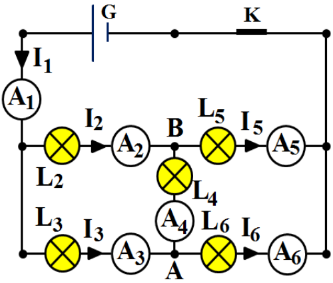
\includegraphics[width=0.58\textwidth]{./img/ex07.png}
  \end{center}


\end{Box2}

Tous les gaz sont considérés comme parfaits : 
\begin{itemize}
\item Toutes les mesures ont été faites à 25°C ;
\item  On rappelle la loi des gaz parfaits : P.V = n.R.T ;
\item  La masse molaire atomique du zinc : $M(Zn) = 65,4 g.mol^{-1}$.
\end{itemize}
\begin{Box2}{Exercice 8 :  la réaction du zinc avec une solution d’acide sulfurique}
	On modélise la réaction du zinc $Zn_{(S)}$ avec une solution d’acide sulfurique $({2H_3O^+}_{(aq)} +{SO_4^{2-}}_{(aq)})$ , par
l’équation chimique suivante :
$$\ce{Zn_{(s)} + 2H_3O^+  <=> Zn^{2+}_{(aq)} + {H_2}_{(g)} + 2H_2O_{(l)}}$$

Pour étudier la cinétique de cette réaction, on introduit dans un ballon de volume constant $V$=$1 L$, une
quantité de masse $m = 0,6 g$ de poudre de Zinc $Zn_{(S)}$, et on y verse à l’instant $t_0 = 0$, un volume $V_a$=$75 mL$ de la solution aqueuse d’acide sulfurique de concentration en ions oxonium $[H_3O^+]$=$0,4 mol/L$.

On mesure la pression P à l’intérieur du ballon, à chaque instant, à l’aide d’un capteur de pression.

\textbf{1. } Soient $n_i(H_3O^+)$ et $n_i(Zn)$ les quantités de matière initiales respectivement des ions oxonium et du
Zn. Dresser le tableau descriptif de la réaction. et Calculer $n_i(H_3O^+)$ et $n_i(Zn)$.

\textbf{2. }Déterminer le réactif limitant et déduire l’avancement maximal  $X_{max}$ de la réaction.

\textbf{3. } Par application de la loi des gaz parfaits, et à l’aide du tableau descriptif précédent, établir
l’expression de l’avancement x(t) de la réaction à un instant t en fonction de R, T, V et $\Delta{P}$, où
$\Delta{P} = P - P_0$, avec $P_0$ la pression initiale mesurée à l’instant  $t_0 = 0$ et P la pression mesurée à l’instant t.

\textbf{4. }Soit $\Delta{P_{max}}= P_{max}  - P_0$ la variation
maximale de la pression et $X_max$
l’avancement maximal de la
réaction. Montrer la relation :
$$x(t) = x_{max}.\frac{\Delta{P}}{\Delta{P_{max}}}$$

Une étude expérimentale a permis
de tracer la courbe de la figure 1,
traduisant les variations de $\Delta{P}$ en
fonction du temps.

\textbf{5. } Trouver graphiquement la valeur du
temps de demi-réaction

  \begin{center}
	  %\vspace{-1.2cm}
	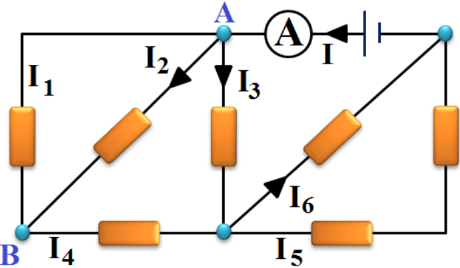
\includegraphics[width=0.58\textwidth]{./img/ex08.png}
  \end{center}

\end{Box2}

\begin{itemize}
	\item Toutes les mesures sont effectuées à 25°C ;
	\item L’expression de la conductance à un instant t est : $G = K.\sum \lambda_i.[X_i]$

		Où $\lambda_i$: Conductivité molaire ionique de l’ion $X_i$.

		k : Constante de la cellule de mesure de valeur k = 0,01 m ;
Le tableau suivant donne les valeurs des conductivités molaires ioniques des ions en
solution : $\lambda(Na^+)$=$5,01.10^{-3}S.m^2/mol$ ;  

$\lambda(HO^-)$=$19,9.10^{-3}S.m^2/mol$ ; $\lambda(HCO_2^-)$=$5,46.10^{-3}S.m^2/mol$
\item On néglige la concentration des ions Hydroniums $H_3O^+$ devant les autres
concentrations des ions présents dans le mélange réactionnel.

\end{itemize}

\begin{Box2}{Exercice 9 :Méthode de mesure de la conductance }
	On verse dans un bécher un volume $V = 2.10^{-4} m^3$ d’une solution $S_B$ d’hydroxyde de
	sodium de concentration molaire $C_B$=$10mol.m^{-3}$, et on y ajoute à l’instant $t_0$ considérée comme origine des temps, une quantité de matière   $n_E$du méthanoate de méthyle égale à la quantité de matière $n_B$ d’hydroxyde de sodium $(n_E$=$n_B)$.

%\begin{wrapfigure}[16]{r}{0.58\textwidth}
%\end{wrapfigure}

	On considère que le volume reste constant $V = 2.10^{-4} m^3$.
	
Une étude expérimentale a permis de tracer la courbe représentative des variations de
la conductance G du mélange en fonction du temps (Figure 1)
On modélise la réaction étudiée par l’équation de réaction suivante :
$${HCO_2CH_3}_{(aq)} + OH^-_{(aq)} \rightarrow {HCO_2^-}_{(aq)} + CH_3OH_{(aq)} $$

\textbf{1. }Faire l’inventaire des ions
présent dans le mélange à un
instant t.

\textbf{2. } construire le tableau descriptif
de l’évolution de
cette transformation.(On notera x l’avancement de la
réaction à l’instant t)

\textbf{3. } Montrer que la conductance G
dans le milieu réactionnel
vérifie la relation : $G = - 0,72 x + 2,5.10^{-3}$ (S).

\textbf{4.} Justifier la décroissance de la conductance G au cours de la réaction.

\textbf{5. }
Déterminer la valeur du temps de demi-réaction t1/2.

  \begin{center}
	  %\vspace{-1.2cm}
	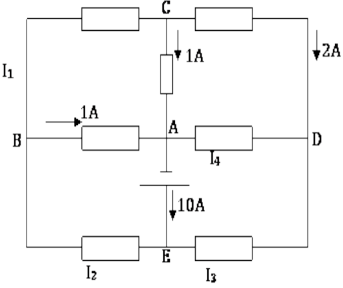
\includegraphics[width=0.58\textwidth]{./img/ex09.png}
  \end{center}



\end{Box2}

\begin{Box2}{Exercice 10 : Etude de la réaction de l’éthanoate d’éthyle avec l’hydroxyde de sodium}

	On introduit, à la date $t = 0$, la quantité de matière $n_0$ de l’éthanoate d’éthyle dans un bécher
	contenant la même quantité de matière $n_0$ d’hydroxyde de sodium $Na^+_{(aq)}$+$HO^-_{(aq)}$ de concentration
	$C_0 $=$10 mol.m^{-3}$ et de volume $V_0$ .

	On considère que le mélange réactionnel obtenu a un volume $V $=$V_0$=$10^{-4} m^3$ .
L’équation associée à la réaction chimique s’écrit :

$${C_4H_8O_2}_{(l)} + HO^-_{(aq)} \rightarrow A^-_{(aq)} + B_{(aq)}$$

\textbf{1. }Dresser le tableau d’avancement de la réaction.

\textbf{2. }On suit l’évolution de la réaction en mesurant la conductivité $\sigma$ du mélange réactionnel à des
instants différents.
Le graphe ci-dessous représente $\sigma{(t)}$ ainsi que la tangente (T) à l’origine.

  \begin{center}
	  %\vspace{-1.2cm}
	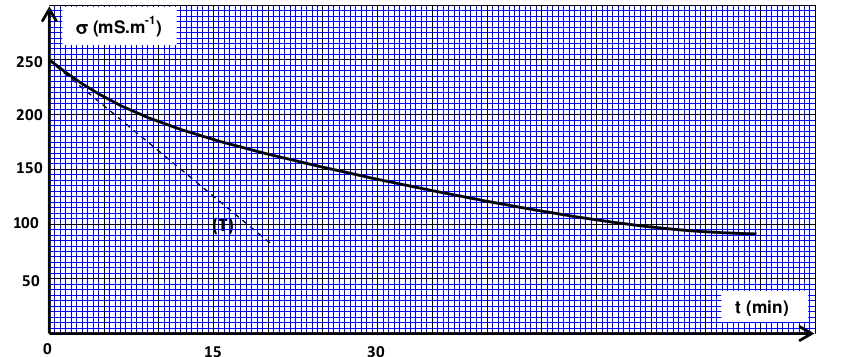
\includegraphics[width=0.8\textwidth]{./img/ex10.png}
  \end{center}

A chaque instant t, l’avancement $x(t)$ peut être calculé par l’expression :
$$x(t) = -6,3.10^{-3}.\sigma(t) + 1,57.10^{-3}$$
avec $\sigma{(t)}$ la conductivité du mélange réactionnel exprimée en
$S/m$ et $x(t)$ en mol. En exploitant la courbe expérimentale :

\textbf{2.1. }Calculer $\sigma_{1/2}$ , la conductivité du mélange réactionnel quand $x = \frac{x_{max}}{2}$ ; $X_{max}$ étant
l’avancement maximal de réaction.

\textbf{2.2. }Trouver, en minutes, le temps de demi-réaction $t_{1/2}$ .

\textbf{2.3. }Déterminer, en $mol.m^{-3}.min^{-1}$ , la vitesse volumique v de la réaction à la date $t=0$ .

\end{Box2}

\begin{Box2}{Exercice 11 : Etude cinétique d’une réaction chimique}
	\emph{L’une des plus anciennes réactions
de synthèse est
la fabrication
du savon. Le savon est un produit
composé de molécules obtenues par réaction chimique, entre un composé organique et une solution
aqueuse d'hydroxyde de sodium.}

Cette partie de l’exercice se propose d’étudier, par conductimétrie, la cinétique de la réaction de
synthèse d’un savon. Cette réaction se produit entre l’éthanoate d’éthyle de formule $CH_3COOC_2H_5$ et une solution aqueuse d’hydroxyde de sodium $Na^+_{(aq)} + HO^-_{(aq)}$ .

À un instant choisi comme origine des dates $t = 0$, on introduit, en excès, l’éthanoate d’éthyle dans un
ballon contenant une quantité de matière $n_0(HO^-)$=$10^{-3}mol$ d’ions hydroxyde. On obtient un
mélange réactionnel ayant un volume $V_0 = 100mL$.

Il se produit, sous une température constante, une réaction modélisée par l’équation chimique
suivante :

\end{Box2}

\begin{Box2}{Exercice 11 : Etude cinétique d’une réaction chimique - (la suite)}
	$${CH_3COOC_2H_5}_{(aq)} + HO^-_{(aq)} \rightarrow CH_3COO^-_{(aq)} + C_2H_5OH_{(aq)} $$

	\textbf{1. } Dresser le tableau d’avancement de cette réaction et déterminer la valeur de l’avancement final $x_f$.sachant que cette réaction est totale.

	\textbf{2. }On mesure, à chaque instant, la conductivité $\sigma$ du
mélange réactionnel.

La courbe de la figure1 donne les variations de la
conductivité du mélange réactionnel en fonction du temps.

La droite (T) représente la tangente à la courbe au point d’abscisse $t_1$=$4min$.

L’expression de la conductivité $\sigma $ du mélange réactionnel
en fonction de l’avancement $x$ de la réaction est :
$\sigma = 0,25-160.x$ où $\sigma$ est exprimée en $S/m$ et x en mol.

\textbf{2.1} Définir le temps de demi-réaction $t_{1/2}$.

\textbf{2.2 }A l’aide de l’expression $\sigma = f(x)$ et de la courbe de la figure1, déterminer la valeur de $t_{ 1/ 2 }$.

\textbf{2.3 }Montrer que la vitesse volumique de la réaction à un instant t s’écrit sous la forme : $$v = -\frac{1}{160.V_0}.\frac{d\sigma}{dt}$$

\textbf{2.4}Déterminer, en $mol.m^{-3}.min^{-1}$ , la valeur $v_1$ de cette vitesse à l’instant $t_1= 4min$.

  \begin{center}
	  %\vspace{-1.2cm}
	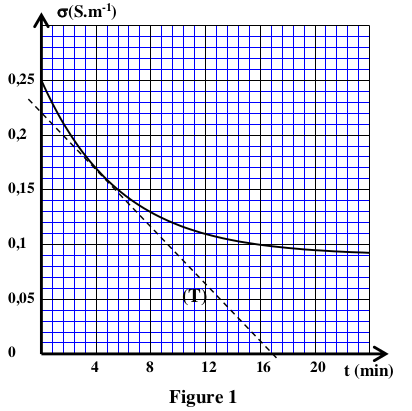
\includegraphics[width=0.57\textwidth]{./img/ex11.png}
  \end{center}



\end{Box2}

\end{document}
